\documentclass[aps,pre,twocolumn,floatfix,groupedaddress,amsmath,amssymb,nofootinbib]{revtex4-2}

\usepackage{graphicx}
\usepackage{booktabs}
\usepackage{xcolor}
\usepackage[colorlinks=true,citecolor=blue,linkcolor=blue,urlcolor=blue]{hyperref}

\newcommand{\ket}[1]{\lvert #1\rangle}
\newcommand{\bra}[1]{\langle #1\rvert}
\newcommand{\Tr}{\operatorname{Tr}}
\newcommand{\W}{\mathcal{W}}

\begin{document}

\title{Collisional spin-coherence battery on a non-collinear
thermoelectric spin valve}

\author{Noufal Jaseem}
\affiliation{Department of Physical Sciences, Indian Institute of Science Education and Research Berhampur, India}
\author{Bitan De}
\affiliation{Institute of Theoretical Physics, Jagiellonian University in Krak\'{o}w, Lojasiewicza 11, 30-348 Krak\'{o}w, Poland}
\author{Parvinder Solanki}
\affiliation{Department of Physics, Indian Institute of Technology Bombay, Powai, Mumbai 400076, India}
\author{Sai Vinjanampathy}
\email{sai@phy.iitb.ac.in}
\affiliation{Department of Physics, Indian Institute of Technology Bombay, Powai, Mumbai 400076, India}
\affiliation{Centre for Quantum Technologies, National University of Singapore, 3 Science Drive 2, 117543 Singapore, Singapore}
\author{Bhaskaran Muralidharan}
\email{bm@ee.iitb.ac.in}
\affiliation{Department of Electrical Engineering, Indian Institute of Technology Bombay, Powai, Mumbai 400076, India}
\date{\today}

\begin{abstract}
We study a Coulomb-blockaded quantum dot coupled to non-collinear magnetic
leads and to a stream of ancilla qubits. The nonequilibrium leads generate
spin coherence in the singly occupied sector. A temperature difference and a
load voltage place the device in a thermoelectric engine regime with positive
electrical output power. Matched-gap exchange collisions then export part of
the spin coherence into the ergotropy of the outgoing ancillas, opening a
second power channel. Using lead-resolved currents built from the same
dissipators that generate the dynamics, we compute cycle-averaged electrical
power and battery charging power at the stroboscopic fixed point. A control
hierarchy---collinear leads, pure dephasing, incoherent exchange, and matched
populations---shows that the battery channel requires coherent exchange, while
the engine branch survives without it. The collisional export map is
summarized by a short companion analysis of impedance-matched harvesting.
The construction is a sequential-tunneling scaffold, not a NEGF theory, and
coherent ergotropy remains an upper bound without a phase reference.
\end{abstract}

\maketitle

\section{Introduction}

Quantum-dot thermoelectric devices convert heat into electrical work at the
nanoscale~\cite{Sothmann2015,Benenti2017,Whitney2014,Josefsson2018}. When the
leads are magnetic and non-collinear, the same nonequilibrium drive that
produces charge current also polarizes the dot spin away from the energy
basis, so a stationary spin coherence appears in the singly occupied
sector~\cite{Splettstoesser2010}. Separately, quantum batteries and
repeated-interaction models ask how fast a nonpassive state can be prepared
and charged~\cite{Allahverdyan2004,AlickiFannes2013,Campaioli2017,Francica2020,Bettmann2023,CollisionalTransmon2025}.

Our question is simple. \emph{Can a non-collinear thermoelectric spin valve
keep a positive electrical output while a collisional tape harvests its spin
coherence as battery ergotropy?} If yes, what controls separate the two
channels?

We answer this in a minimal Coulomb-blockade model with sequential tunneling
to polarized leads and resonant exchange collisions with ground-state
ancillas. Three results structure the paper. (i)~In a near-degenerate
window, non-collinearity produces a usable spin coherence, while collinear
leads and large level splitting suppress it. (ii)~A temperature bias together
with a load voltage places the device on a thermoelectric engine branch with
$P_{\mathrm{el}}>0$. (iii)~Coherent exchange collisions open a second channel
$P_{\mathrm{erg}}=r\W_A$, which vanishes under incoherent exchange, collinear
leads, or no collision.

We do not claim that exporting coherence restores a higher collinear
electrical power. We treat electrical and battery powers as coexisting
outputs. We report total ancilla ergotropy as an upper bound: without a
phase reference the coherent part is not free under energy-preserving
discharge~\cite{Lostaglio2015,Francica2020}.

\section{Model}

\subsection{Dot and leads}

The strong-blockade Fock space is
$\{\ket{0},\ket{\uparrow},\ket{\downarrow}\}$ with
\begin{equation}
H_D=\varepsilon(n_\uparrow+n_\downarrow)+\frac{\Delta}{2}(n_\uparrow-n_\downarrow).
\end{equation}
Each lead $\alpha\in\{L,R\}$ has broadening matrix $\Gamma_\alpha$ with
polarization $p_\alpha$ and, for the right lead, tilt $(\theta_R,\phi_R)$.
Temperatures $T_L>T_R$ and chemical potentials $\mu_L,\mu_R$ define the bias
$V=\mu_L-\mu_R$. Between collisions the reduced density matrix evolves under
a sequential-tunneling Liouvillian built from spinor jump operators of
$\Gamma_\alpha$ (Appendix~\ref{app:leads}). The generator is completely
positive by construction. It is \emph{not} a derived Redfield equation; all
claims below are inside this scaffold.

\subsection{Collisions}

A second, permanently occupied ancilla qubit with gap $\Delta_A=\Delta$
interacts for a time $\tau$ through
\begin{equation}
H_{\mathrm{int}}=\hbar g\bigl(
\ket{\uparrow_D\downarrow_A}\bra{\downarrow_D\uparrow_A}+\mathrm{h.c.}\bigr),
\end{equation}
so $\theta=g\tau$. On the active block the free Hamiltonian is resonant and
$[H_D+H_A,H_{\mathrm{int}}]=0$. Fresh ancillas arrive with period $T$ and
excited population $\alpha$ (usually $\alpha=0$). The stroboscopic map is
waiting under the leads, then one collision. Observables are evaluated at
the periodic fixed point.

\subsection{Bookkeeping}

Lead-tagged dissipators define
\begin{align}
J_{N,\alpha}&=\mathrm{Re}\,\Tr\!\big[N_D\,\mathcal L_\alpha(\rho)\big],\\
J_{E,\alpha}&=\mathrm{Re}\,\Tr\!\big[H_D\,\mathcal L_\alpha(\rho)\big],\\
J_{Q,\alpha}&=J_{E,\alpha}-\mu_\alpha J_{N,\alpha},
\end{align}
with $N_D=\mathrm{diag}(0,1,1)$. Currents are cycle-averaged over the
waiting interval and divided by $T$ (leads off during the collision). We
set
\begin{equation}
I\equiv \bar J_{N,L},\qquad
P_{\mathrm{el}}\equiv -(\mu_L-\mu_R)I,
\end{equation}
so $P_{\mathrm{el}}>0$ is electrical \emph{output}. The battery channel is
\begin{equation}
P_{\mathrm{erg}}=r\,\W_A,\qquad r=1/T,
\end{equation}
where $\W_A$ is the ergotropy of the outgoing ancilla. Continuous NESS
checks satisfy $J_{N,L}+J_{N,R}\approx0$ to numerical precision.

\section{Spin resource without collisions}

Figure~\ref{fig:resource} maps the continuous-lead steady state in the
engine window of temperatures and chemical potentials used below. Spin
coherence $|C|=|\rho_{\uparrow\downarrow}|$ is large at small $\Delta$ and
intermediate tilt, and vanishes for collinear leads. Electrical power
$P_{\mathrm{el}}$ is positive over a connected region of $(\Delta,\theta_R)$.
Thus the same nonequilibrium drive that supports thermoelectric operation
also hosts a harvestable spin resource---without an engineered coherence
target.

\begin{figure}[t]
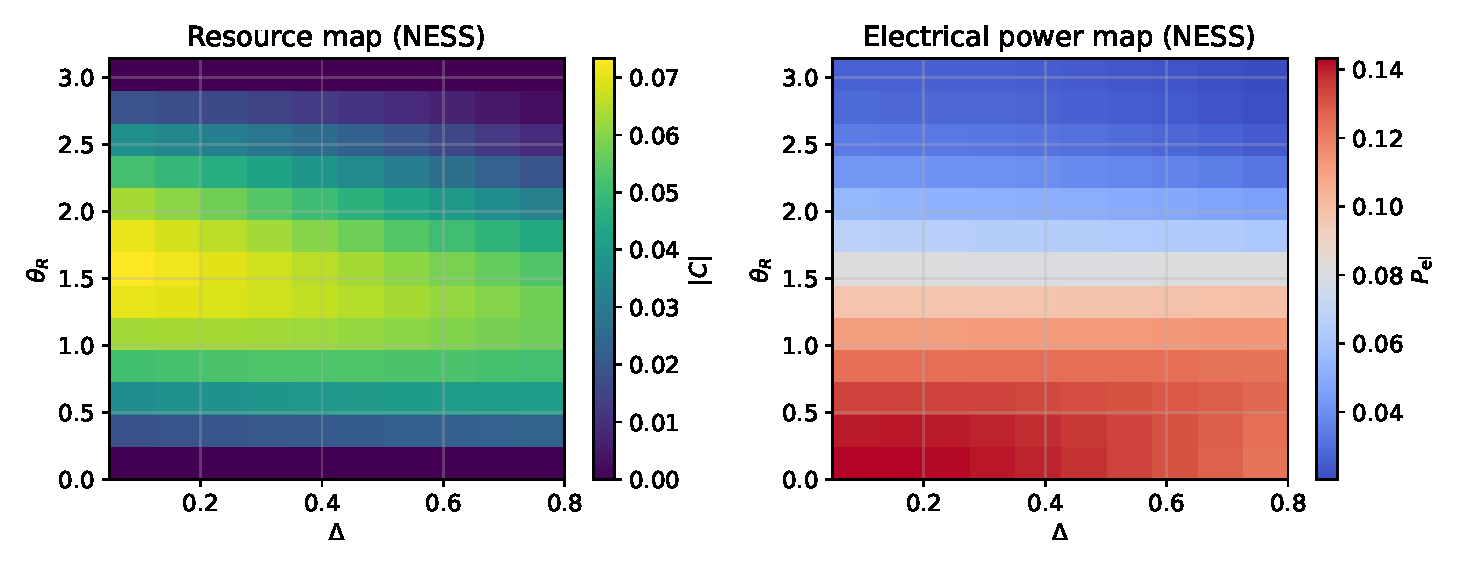
\includegraphics[width=\linewidth]{figures/fig_resource_map.pdf}
\caption{NESS resource and electrical power versus level splitting $\Delta$
and right-lead tilt $\theta_R$ at fixed $(T_L,T_R,\mu_L,\mu_R,p)$. Left:
$|C|$. Right: $P_{\mathrm{el}}$.}
\label{fig:resource}
\end{figure}

\section{Thermoelectric engine branch}

Fix temperatures $T_L>T_R$ and scan the load $V=\mu_L-\mu_R$.
Figure~\ref{fig:load} shows a clear engine branch at negative $V$: the
thermocurrent runs against the load, so $P_{\mathrm{el}}>0$, while $|C|$
remains finite. At the representative working point
\begin{equation}
\begin{aligned}
&(T_L,T_R)=(2.0,0.25),\quad
(\mu_L,\mu_R)=(-0.3,0.3),\\
&\varepsilon=1.0,\ \Delta=0.2,\ \theta_R=0.6,\ p_L=p_R=0.9,
\end{aligned}
\end{equation}
the continuous NESS has $P_{\mathrm{el}}\approx0.132$ and $|C|\approx0.042$.
A diagnostic efficiency $\eta\approx P_{\mathrm{el}}/J_{Q,L}$ on the engine
branch is reported only as a scaffold check, not as a Carnot-tight result.

\begin{figure}[t]
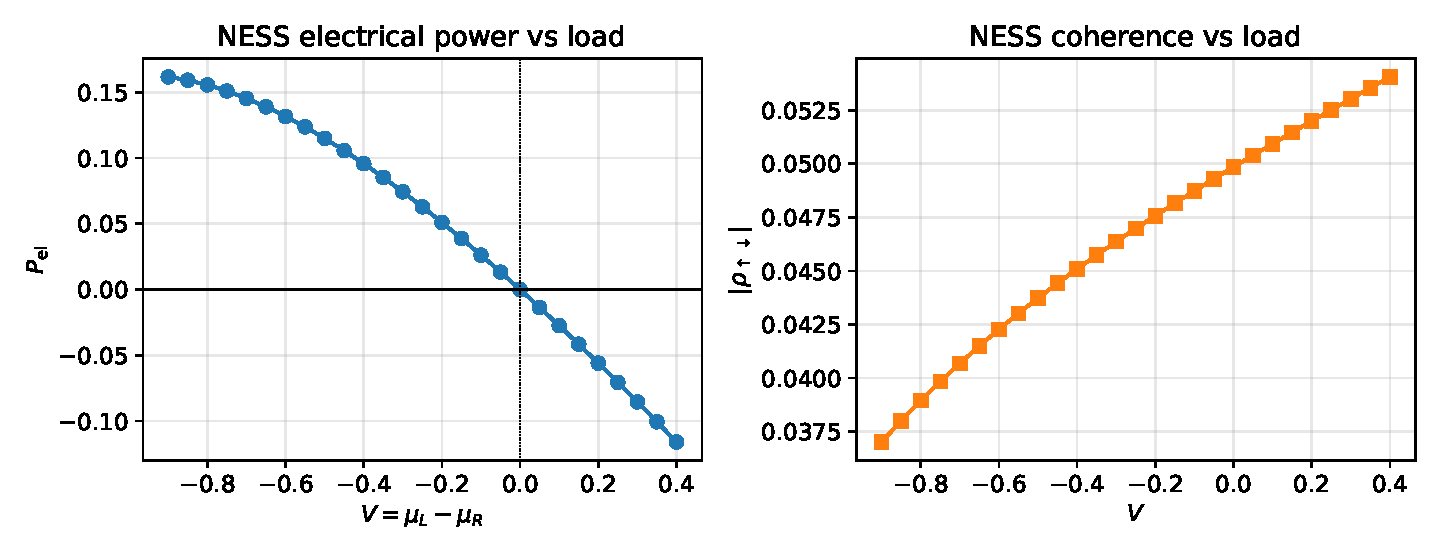
\includegraphics[width=\linewidth]{figures/fig_load_sweep.pdf}
\caption{NESS load sweep. Left: electrical output power versus
$V=\mu_L-\mu_R$. Right: spin coherence. The engine branch is the region
with $P_{\mathrm{el}}>0$.}
\label{fig:load}
\end{figure}

\section{Collisional battery channel}

We now add collisions at exchange angle $\theta\approx0.45$ and scan the
collision rate $r=1/T$ on the engine window
(Fig.~\ref{fig:dual}). Electrical output stays positive for all rates in the
scan, $P_{\mathrm{el}}\in[0.097,0.128]$. The battery power $P_{\mathrm{erg}}$
is smaller, of order $10^{-4}$--$10^{-5}$, because the matched gap $\Delta$
sets the battery energy scale, but it is strictly positive for coherent
exchange and peaks at higher $r$. Residual coherence remains of order a few
percent. Thus the device keeps an engine branch while a second channel
charges the ancilla tape.

\begin{figure}[t]
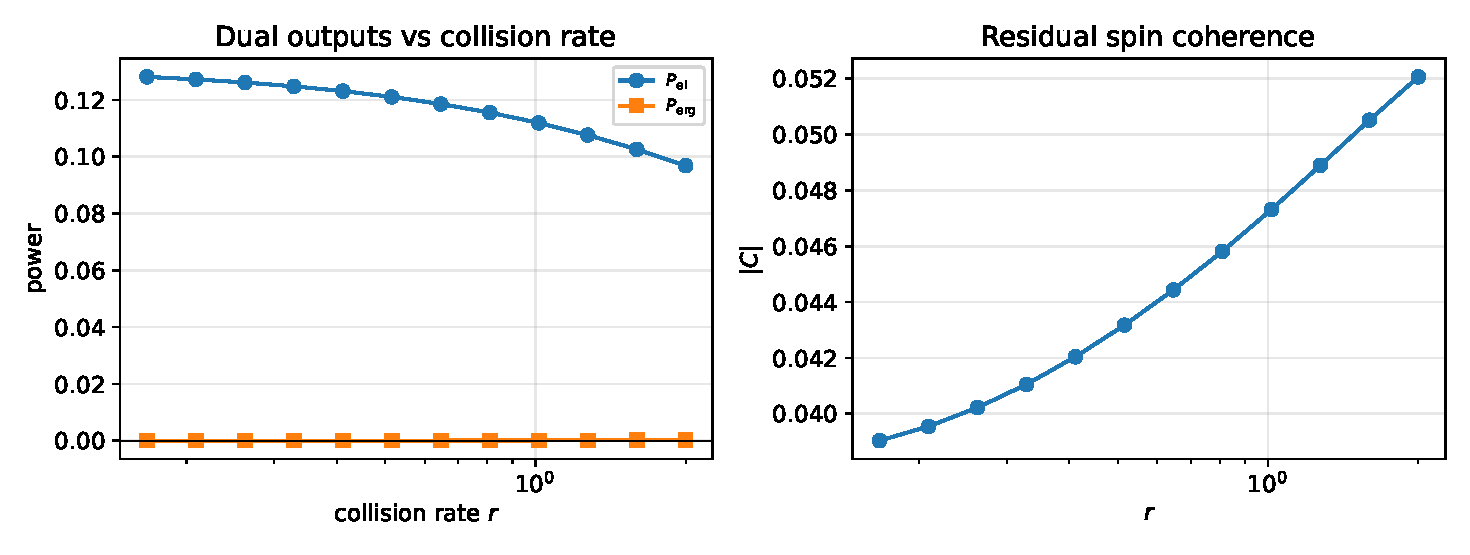
\includegraphics[width=\linewidth]{figures/fig_dual_rate.pdf}
\caption{Stroboscopic fixed point on the engine window. Left: dual powers
versus collision rate. Right: residual spin coherence. $P_{\mathrm{el}}$
stays positive; $P_{\mathrm{erg}}$ opens only with collisions.}
\label{fig:dual}
\end{figure}

\begin{figure}[t]
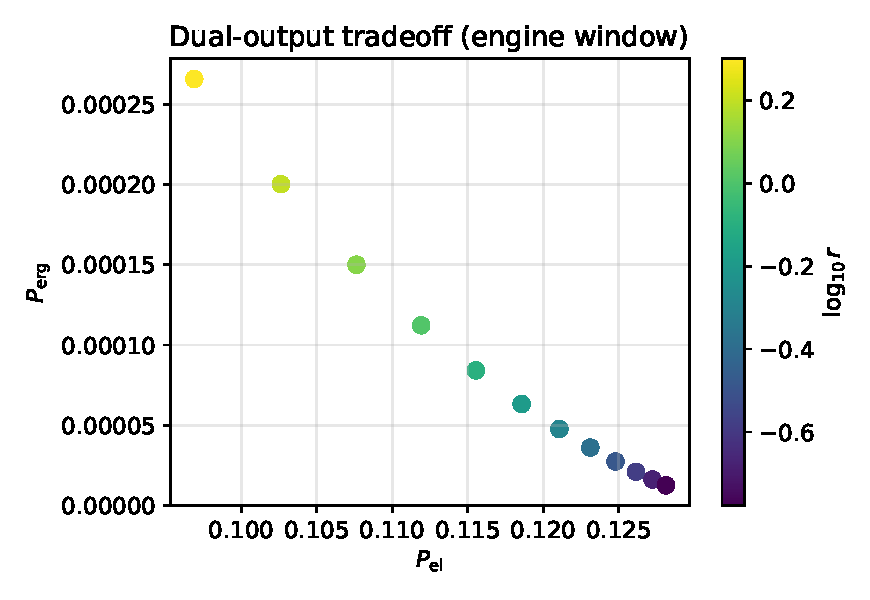
\includegraphics[width=0.9\linewidth]{figures/fig_tradeoff.pdf}
\caption{Tradeoff scan $(P_{\mathrm{el}},P_{\mathrm{erg}})$ along the rate
path. Color encodes $\log_{10}r$.}
\label{fig:tradeoff}
\end{figure}

\section{Control hierarchy}

Figure~\ref{fig:controls} compares protocols at fixed $(T,\theta)$.
Coherent exchange produces $P_{\mathrm{erg}}>0$ with $\W_A$ purely coherent
for ground-state ancillas. Incoherent exchange (spin dephasing before the
unitary), no collision, collinear leads, pure dephasing, and
$\alpha=1/2$ all give $\W_{\mathrm{coh}}=0$ (hence $P_{\mathrm{erg}}=0$ or
only population ergotropy). Matched-population ancillas strongly suppress
the battery channel in this window. Collinear and dephasing protocols can
slightly raise $P_{\mathrm{el}}$, so local coherence is not required for
electrical output and can even cost a small fraction of it. The battery
channel, by contrast, requires coherent non-collinear exchange.

\begin{figure}[t]
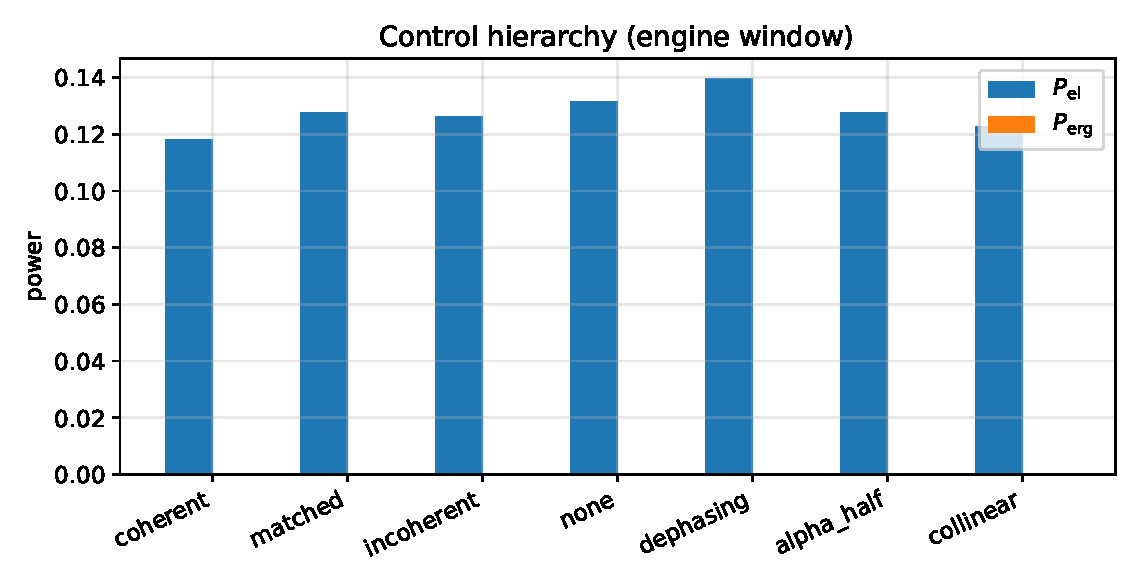
\includegraphics[width=\linewidth]{figures/fig_controls.pdf}
\caption{Control hierarchy at fixed period and exchange angle on the engine
window. Only coherent collisions open a clear battery channel.}
\label{fig:controls}
\end{figure}

\section{Companion export lemma}

The export step is the same matched-gap collision analyzed in a V-type
companion model: an affine renewal of coherence between collisions yields an
impedance-matching optimum $\Gamma_{\mathrm{ext}}=r(1-\cos\theta)\simeq\gamma_C$
for the charging power, with a flat small-angle plateau and a closed
finite-precession factor. In the spin valve the ``regrowth rate'' is set by
the leads rather than an engineered $c_0$. We therefore use the companion
results as lemmas for the collision algebra and accessibility bookkeeping,
not as a substitute for transport.

\section{Discussion}

The main story is dual output in a sequential-tunneling non-collinear
valve: thermoelectric electrical power plus a collisional coherence battery.
The battery channel is small compared with $P_{\mathrm{el}}$ at the present
parameters, which is expected for a small matched gap. The honest reading is
not that harvesting repairs the collinear engine, but that non-collinearity
creates an additional resource that can be exported without destroying the
engine branch.

Limits are explicit. Currents come from the sequential-tunneling generator,
not NEGF. Ancilla preparation free energy is not subtracted. Coherent
ergotropy of a single outgoing qubit is an upper bound without a phase
reference~\cite{Lostaglio2015}. Minimal thermal-qubit repeated-interaction
no-go results~\cite{NoGo2026} concern a different setup; they are cited only
as background for collision models.

\section{Conclusion}

A non-collinear Coulomb-blockade spin valve can operate as a thermoelectric
engine while a tape of ancillas harvests its spin coherence through resonant
exchange collisions. Lead-resolved, cycle-averaged currents keep
$P_{\mathrm{el}}>0$ on the chosen window for all collision rates we scanned.
A control hierarchy attributes the battery channel to coherent exchange.
The result is a dual-output picture of nonequilibrium spin-valve resources,
with the collisional map controlled by a short companion analysis of
impedance-matched harvesting.

\begin{acknowledgments}
N.J.\ developed the numerical engine layer and the dual-output analysis.
S.V.\ and B.M.\ proposed coupling a coherence-generating transport device to
an ancilla tape. All authors contributed to the interpretation and the
manuscript.
\end{acknowledgments}

\appendix

\section{Lead generator and currents}
\label{app:leads}

For each lead $\alpha$, $\Gamma_\alpha$ is diagonalized in spin space. Each
eigenchannel with weight $\lambda$ defines a spinor jump operator
$L_+=c_\uparrow\ket{\uparrow}\bra{0}+c_\downarrow\ket{\downarrow}\bra{0}$
with Fermi factors at the spinor energy. The full Liouvillian is
$-i[H_D,\cdot]$ plus Lindblad dissipators for all channels. Particle and
energy currents are
$J_{N,\alpha}=\mathrm{Re}\,\Tr[N_D\mathcal L_\alpha(\rho)]$ and
$J_{E,\alpha}=\mathrm{Re}\,\Tr[H_D\mathcal L_\alpha(\rho)]$. Cycle averages
integrate these currents over the waiting interval and divide by $T$.

\section{Collision channel}

On the active block the exchange unitary is a partial iSWAP of angle
$\theta$. Tracing a diagonal ancilla reproduces the companion map for the
doublet variables $(s,d,C)$ in the singly occupied sector, with an
occupation penalty from empty and doubly blocked weight outside that sector.
At $\alpha=1/2$ the local ancilla coherence vanishes and only population
ergotropy can remain.

\bibliography{references}

\end{document}
